\documentclass[journal=jacsat,manuscript=article]{achemso}
\SectionNumbersOn
\usepackage{multicol}
\usepackage{graphicx}% Include figure files
\usepackage{graphicx}% Include figure files
\usepackage{dcolumn}% Align table columns on decimal point
\usepackage{bm}% bold math
%\usepackage[mathlines]{lineno}% Enable numbering of text and display math
%\linenumbers\relax % Commence numbering lines
\usepackage{pgffor}
\usepackage[utf8]{inputenc}
\usepackage[T1]{fontenc}
\usepackage{mathptmx}
\usepackage{listings}
\lstset{language=Python}
\usepackage{rotating} % Rotating table
\usepackage{caption}
\usepackage{subcaption}

\usepackage{color}
\usepackage{dcolumn} % decimal align in tables
\usepackage{bm} % bold math
\usepackage{graphicx}
\usepackage{multirow} % for table cells to span rows
\usepackage{pifont} % for checkmarks
\usepackage{epsfig}
\usepackage{amsmath} % matrix
% \usepackage{subfigure}
\usepackage{float}
\usepackage{booktabs}
\usepackage{tabularx}
\usepackage{natbib}
\usepackage{gensymb}
\setlength{\paperwidth}{8.5in}
\setlength{\paperheight}{11.0in}
\usepackage{rotating}
\usepackage{threeparttable}
\usepackage{comment}
%for corrections
\usepackage[normalem]{ulem}
% \usepackage{xr-hyper}

%%%%%%%%%%%%%%%%%%%%%%%%%%%%%%%%%%%%%%%%%%%%%%%%%%%%%%%%%%%%%%%%%%%%%
%% Place any additional packages needed here.  Only include packages
%% which are essential, to avoid problems later. Do NOT use any
%% packages which require e-TeX (for example etoolbox): the e-TeX
%% extensions are not currently available on the ACS conversion
%% servers.
%%%%%%%%%%%%%%%%%%%%%%%%%%%%%%%%%%%%%%%%%%%%%%%%%%%%%%%%%%%%%%%%%%%%%
\usepackage[version=3]{mhchem} % Formula subscripts using \ce{}
\usepackage{xcolor}
% \usepackage{xr-hyper}
\usepackage{xr-hyper}
\usepackage{xr}



% \usepackage{hyperref}
\usepackage{amsmath,amssymb,amsthm}
\usepackage{mathtools,physics}


\usepackage{subcaption}
\usepackage{caption}
% \usepackage{titling}
%%%%%%%%%%%%%%%%%%%%%%%%%%%%%%%%%%%%%%%%%%%%%%%%%%%%%%%%%%%%%%%%%%%%%
%% If issues arise when submitting your manuscript, you may want to
%% un-comment the next line.  This provides information on the
%% version of every file you have used.
%%%%%%%%%%%%%%%%%%%%%%%%%%%%%%%%%%%%%%%%%%%%%%%%%%%%%%%%%%%%%%%%%%%%%
%%\listfiles

%%%%%%%%%%%%%%%%%%%%%%%%%%%%%%%%%%%%%%%%%%%%%%%%%%%%%%%%%%%%%%%%%%%%%
%% Place any additional macros here.  Please use \newcommand* where
%% possible, and avoid layout-changing macros (which are not used
%% when typesetting).
%%%%%%%%%%%%%%%%%%%%%%%%%%%%%%%%%%%%%%%%%%%%%%%%%%%%%%%%%%%%%%%%%%%%%


% Add line numbers, as requested by Nature
\usepackage{lineno}
% \linenumbers





%%%% HELPER CODE FOR DEALING WITH EXTERNAL REFERENCES
% (from an answer by cyberSingularity at http://tex.stackexchange.com/a/69832/226)
%%%

\usepackage{xcite}

%%%%%%%%%%%%%%%%%%%%%%%%%%%%%%%%%%%%%%%%%%%%%%%%%%%%%%%%%%%%%%%%%%%%%%%%
%----Helper code for dealing with external references----
% (by cyberSingularity at http://tex.stackexchange.com/a/69832/226)

\usepackage{xr}
\makeatletter

\newcommand*{\addFileDependency}[1]{% argument=file name and extension
	\typeout{(#1)}% latexmk will find this if $recorder=0
	% however, in that case, it will ignore #1 if it is a .aux or 
	% .pdf file etc and it exists! If it doesn't exist, it will appear 
	% in the list of dependents regardless)
	%
	% Write the following if you want it to appear in \listfiles 
	% --- although not really necessary and latexmk doesn't use this
	%
	\@addtofilelist{#1}
	%
	% latexmk will find this message if #1 doesn't exist (yet)
	\IfFileExists{#1}{}{\typeout{No file #1.}}
}\makeatother

\newcommand*{\myexternaldocument}[1]{%
	\externaldocument{#1}%
	\addFileDependency{#1.tex}%
	\addFileDependency{#1.aux}%
}
%------------End of helper code--------------

% put all the external documents here!

\newcommand{\siref}[1]{S\ref{#1}}
%%%%%%%%%%%%%%%%%%%%%%%%%%%%%%%%%%%%%%%%%%%%%%%%%%%%%%%%%%%%%%%%%%%%%%%%


%%%%%%%%%%%%%%%%%%%%%%%%%%%%%%%%%%%%%%%%%%%%%%%%%%%%%%%%%%%%%%%%%%%%%
%% The document title should be given as usual. Some journals require
%% a running title from the author: this should be supplied as an
%% optional argument to \title.
%%%%%%%%%%%%%%%%%%%%%%%%%%%%%%%%%%%%%%%%%%%%%%%%%%%%%%%%%%%%%%%%%%%%%
\title{A Combinatorial Search of Parameterized Quantum Circuit Learning for Chemical Applications}
%%%%%%%%%%%%%%%%%%%%%%%%%%%%%%%%%%%%%%%%%%%%%%%%%%%%%%%%%%%%%%%%%%%%%
%% Meta-data block
%% ---------------
%% Each author should be given as a separate \author command.
%%
%% Corresponding authors should have an e-mail given after the author
%% name as an \email command. Phone and fax numbers can be given
%% using \phone and \fax, respectively; this information is optional.
%%
%% The affiliation of authors is given after the authors; each
%% \affiliation command applies to all preceding authors not already
%% assigned an affiliation.
%%
%% The affiliation takes an option argument for the short name.  This
%% will typically be something like "University of Somewhere".
%%
%% The \altaffiliation macro should be used for new address, etc.
%% On the other hand, \alsoaffiliation is used on a per author basis
%% when authors are associated with multiple institutions.
%%%%%%%%%%%%%%%%%%%%%%%%%%%%%%%%%%%%%%%%%%%%%%%%%%%%%%%%%%%%%%%%%%%%%
\author{Grier M. Jones}
\affiliation[UTSG ECE]{
	The Edward S. Rogers Sr. Department of Electrical and Computer Engineering, 
	University of Toronto, 
	10 Kings College Road, Toronto, Ontario, 
	Canada M5S 3G4}
\alsoaffiliation[UTM CHEM]{
	Department of Chemical and Physical Sciences, 
	University of Toronto Mississauga, 
	3359 Mississauga Road, Mississauga, Ontario, 
	Canada L5L 1C6}

\author{Nick Taylor}
\affiliation[UTSG ECE]{
	The Edward S. Rogers Sr. Department of Electrical and Computer Engineering, 
	University of Toronto, 
	10 Kings College Road, Toronto, Ontario, 
	Canada M5S 3G4}

\author{Viki Kumar Prasad}
\affiliation[UTSG ECE]{
	The Edward S. Rogers Sr. Department of Electrical and Computer Engineering, 
	University of Toronto, 
	10 Kings College Road, Toronto, Ontario, 
	Canada M5S 3G4}
\alsoaffiliation[UTM CHEM]{
	Department of Chemical and Physical Sciences, 
	University of Toronto Mississauga, 
	3359 Mississauga Road, Mississauga, Ontario, 
	Canada L5L 1C6}



\author{Ulrich Fekl}
\affiliation[UTM CHEM]{
	Department of Chemical and Physical Sciences, 
	University of Toronto Mississauga, 
	3359 Mississauga Road, Mississauga, Ontario, 
	Canada L5L 1C6}
\email{ulrich.fekl@utoronto.ca}

\author{Hans-Arno Jacobsen}
\affiliation[UTSG ECE]{
	The Edward S. Rogers Sr. Department of Electrical and Computer Engineering, 
	University of Toronto, 
	10 Kings College Road, Toronto, Ontario, 
	Canada M5S 3G4}
\email{jacobsen@eecg.toronto.edu}
%%%%%%%%%%%%%%%%%%%%%%%%%%%%%%%%%%%%%%%%%%%%%%%%%%%%%%%%%%%%%%%%%%%%%
%% Some journals require a list of abbreviations or keywords to be
%% supplied. These should be set up here, and will be printed after
%% the title and author information, if needed.
%%%%%%%%%%%%%%%%%%%%%%%%%%%%%%%%%%%%%%%%%%%%%%%%%%%%%%%%%%%%%%%%%%%%%
\abbreviations{}
\keywords{American Chemical Society, \LaTeX}

%%%%%%%%%%%%%%%%%%%%%%%%%%%%%%%%%%%%%%%%%%%%%%%%%%%%%%%%%%%%%%%%%%%%%
%% The manuscript does not need to include \maketitle, which is
%% executed automatically.
%%%%%%%%%%%%%%%%%%%%%%%%%%%%%%%%%%%%%%%%%%%%%%%%%%%%%%%%%%%%%%%%%%%%%
\newcommand{\R}{\mathbb{R}}

\begin{document}

\newpage
\section*{Electronic Supplementary Information}
\setcounter{page}{1}
\renewcommand{\thepage}{S-\arabic{page}}


\subsection*{Table of Contents}
\begin{table}[H]
	\centering
	\begin{tabular}{|c|c|}
		\hline
		\textbf{Section} & \textbf{Page} \\
		\hline
		\siref{section:bse49_molrep}  BSE49: Molecular Representations & \pageref{section:bse49_molrep} \\
		\hline
		\siref{section:feature_reduction} Classical Feature Reduction& \pageref{section:feature_reduction} \\ 
		\hline
		\siref{section:DDCC_fake}  DDCC Fake Quebec & \pageref{section:DDCC_fake} \\
		\hline
		S3. & \pageref{section:section3} \\
		\hline
	\end{tabular}
	\label{tab:my_label}
\end{table}
\setcounter{figure}{0}
\renewcommand{\figurename}{Figure}
\renewcommand{\thefigure}{S\arabic{figure}}
\newpage
\section{BSE49: Molecular Representations}\label{section:bse49_molrep}

\begin{figure}[H]
	\centering	
	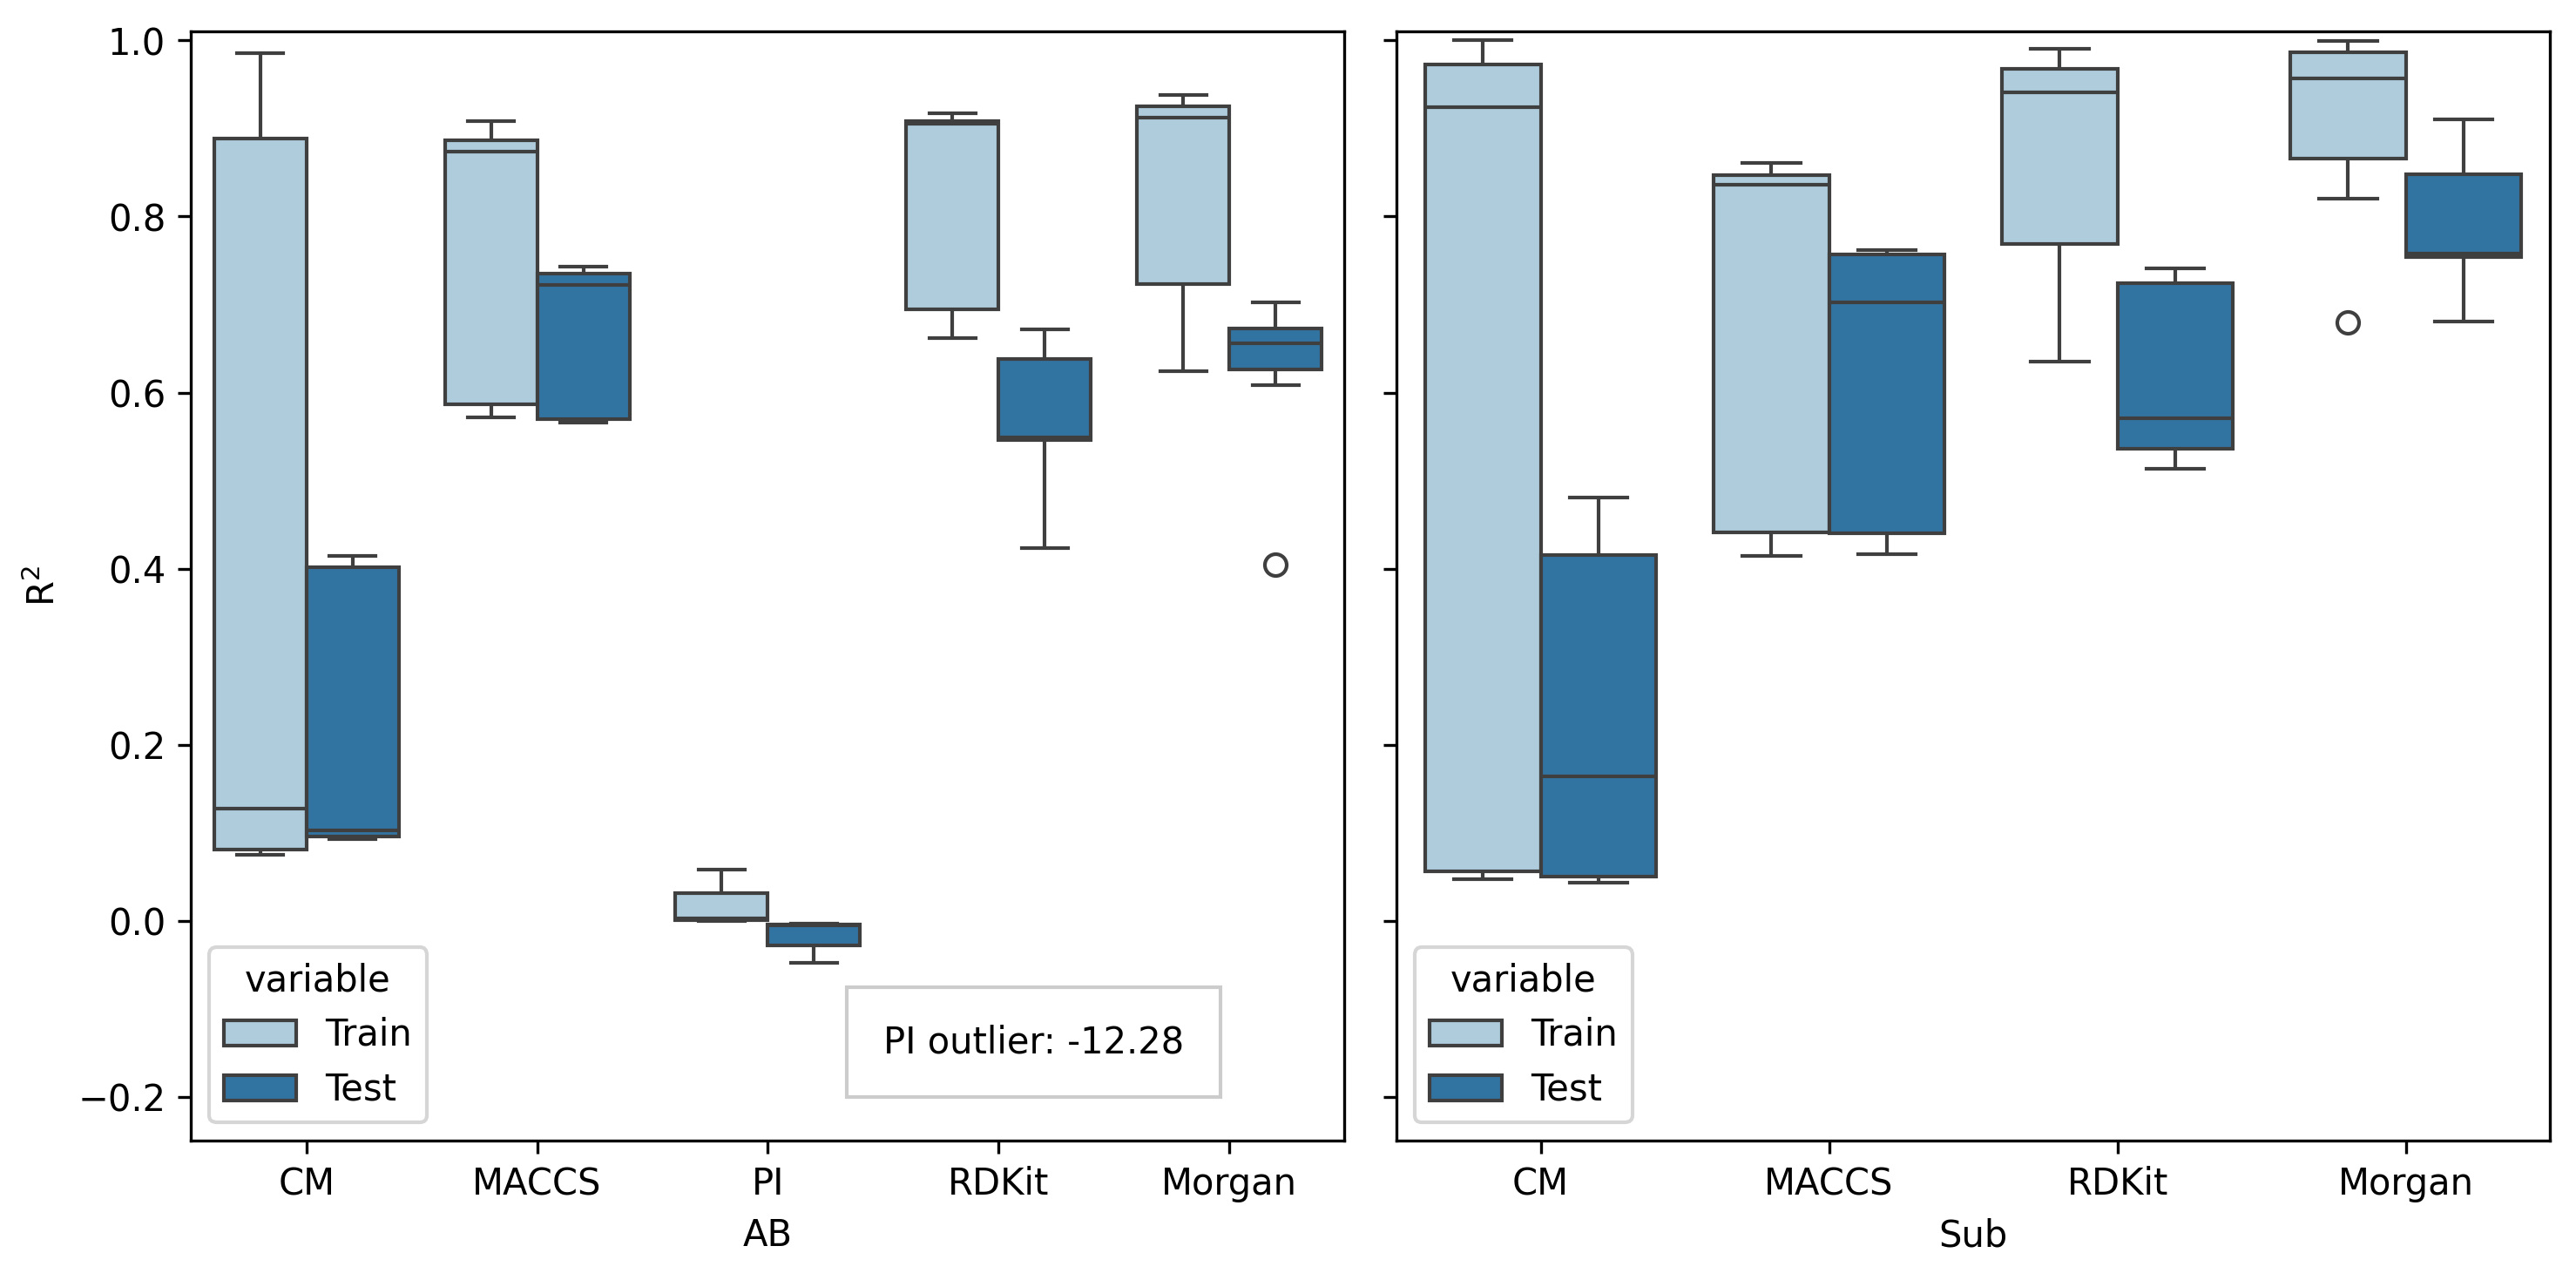
\includegraphics[width=\linewidth]{../images/BSE/classical/classical_molrepfig.png}
	\caption{Coulomb matrices (CMs), Molecular ACCess Systems (MACCS), persistence images (PIs), RDKit and Morgan fingerprints. Performance of a diverse set of molecular representations R$^{2}$}
	\label{fig:classical_molrepfig}
\end{figure}


\section{Classical Feature Reduction}\label{section:feature_reduction}

\begin{figure}[H]
	\centering	
	\begin{subfigure}[b]{0.49\textwidth}
		\centering
		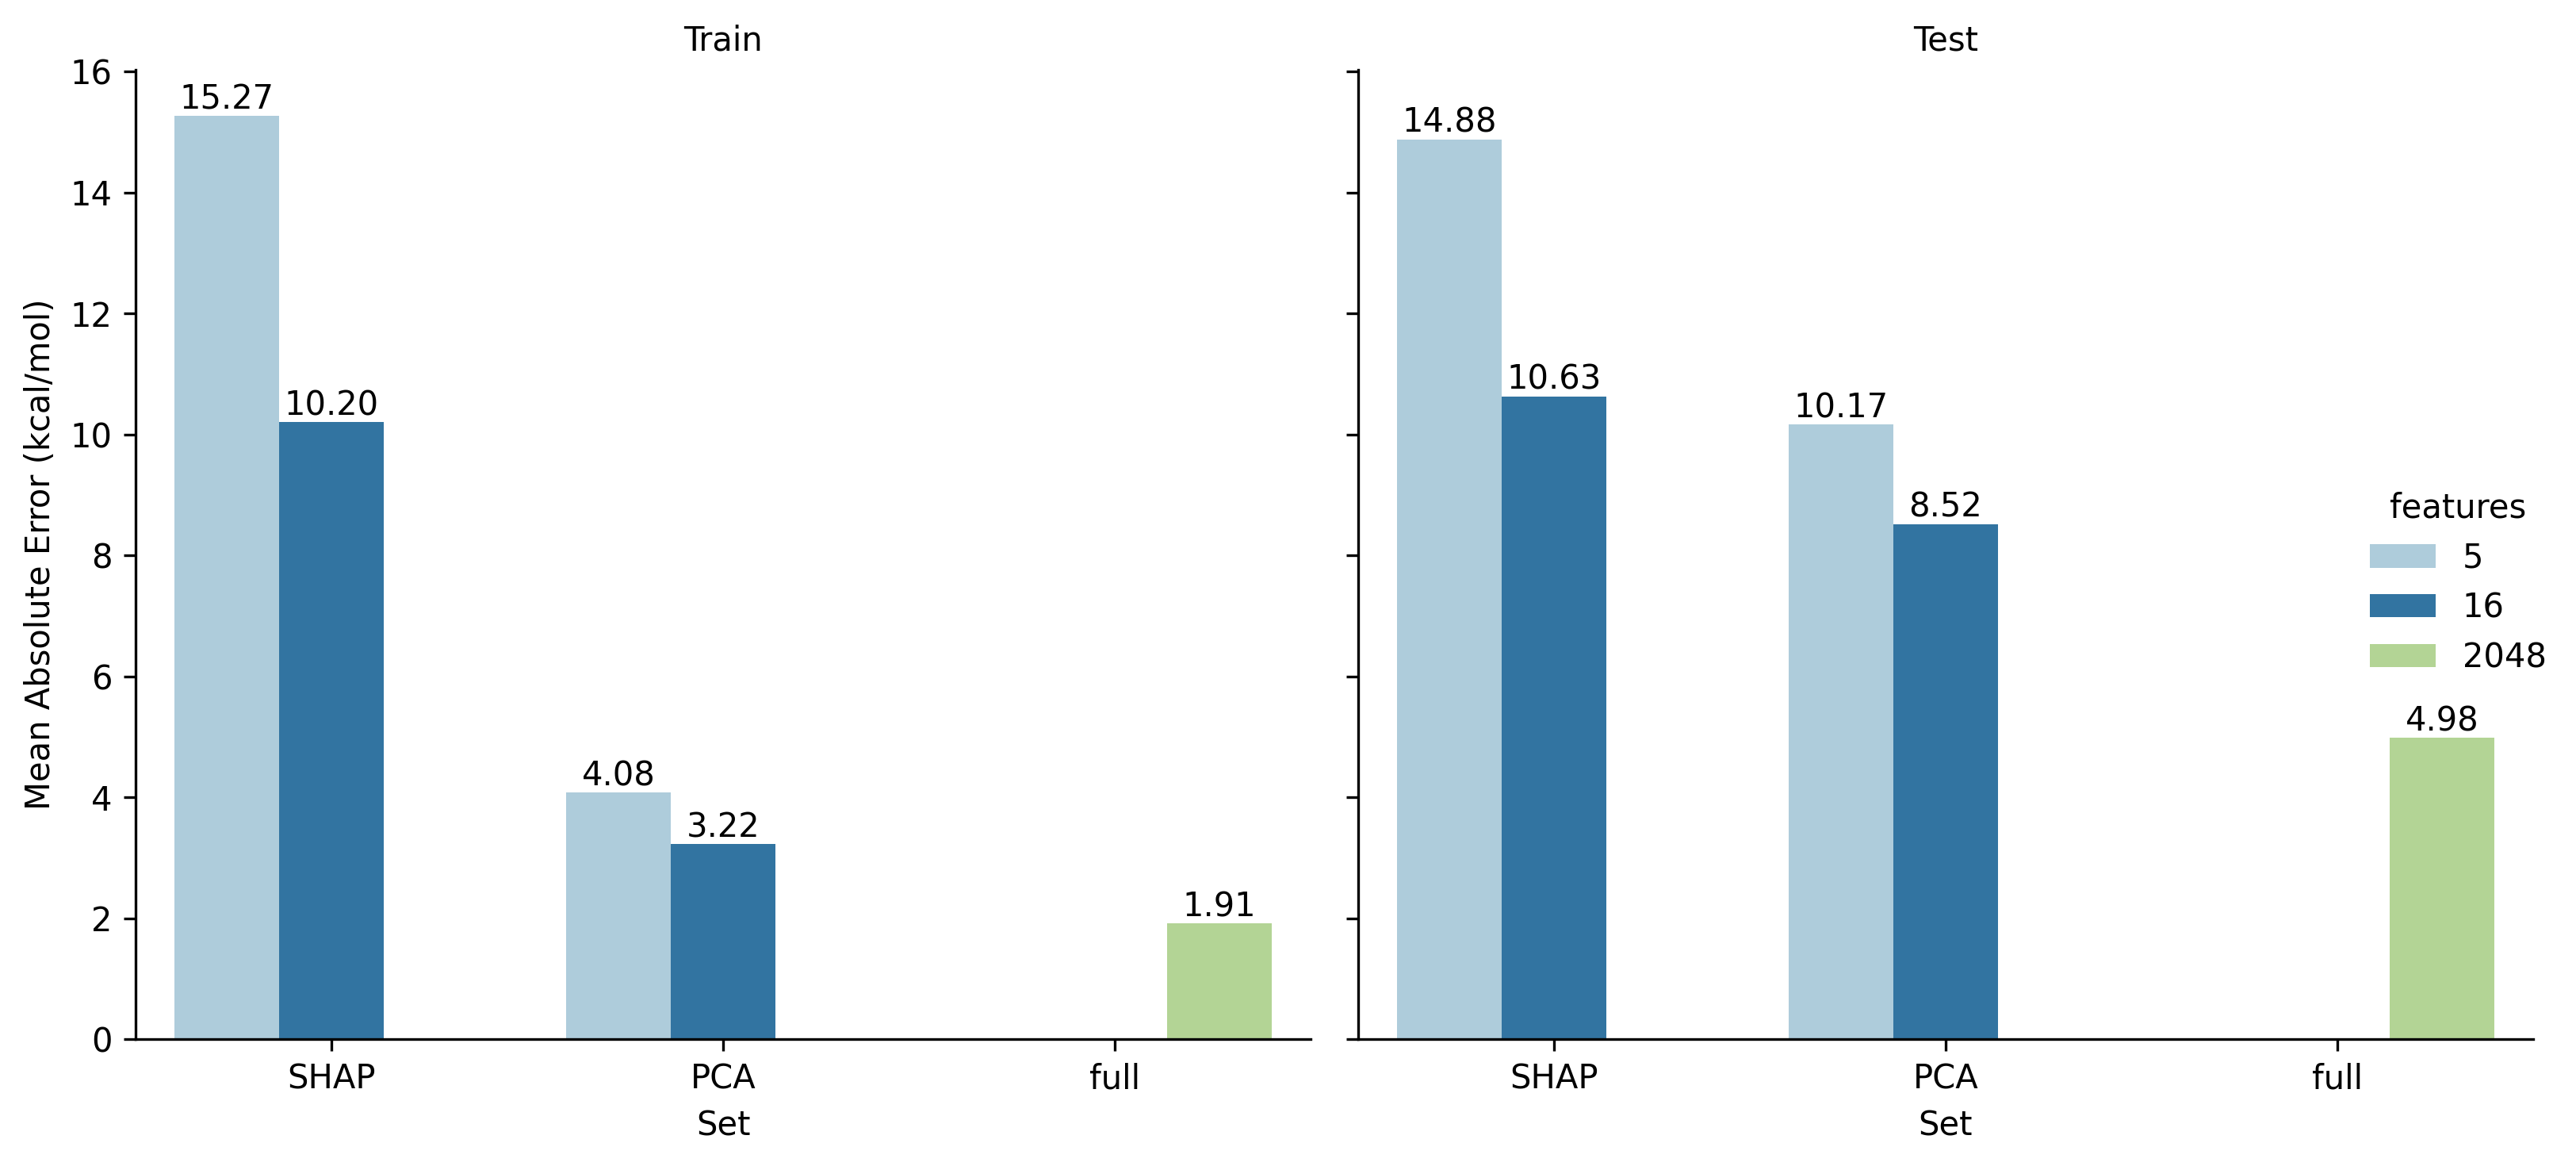
\includegraphics[width=\textwidth]{../images/BSE/classical_features_MAE.png}
		\caption{}
		\label{fig:BSE_bse_classical_features_MAE}
	\end{subfigure}
	\hfill		
	\begin{subfigure}[b]{0.49\textwidth}
		\centering
		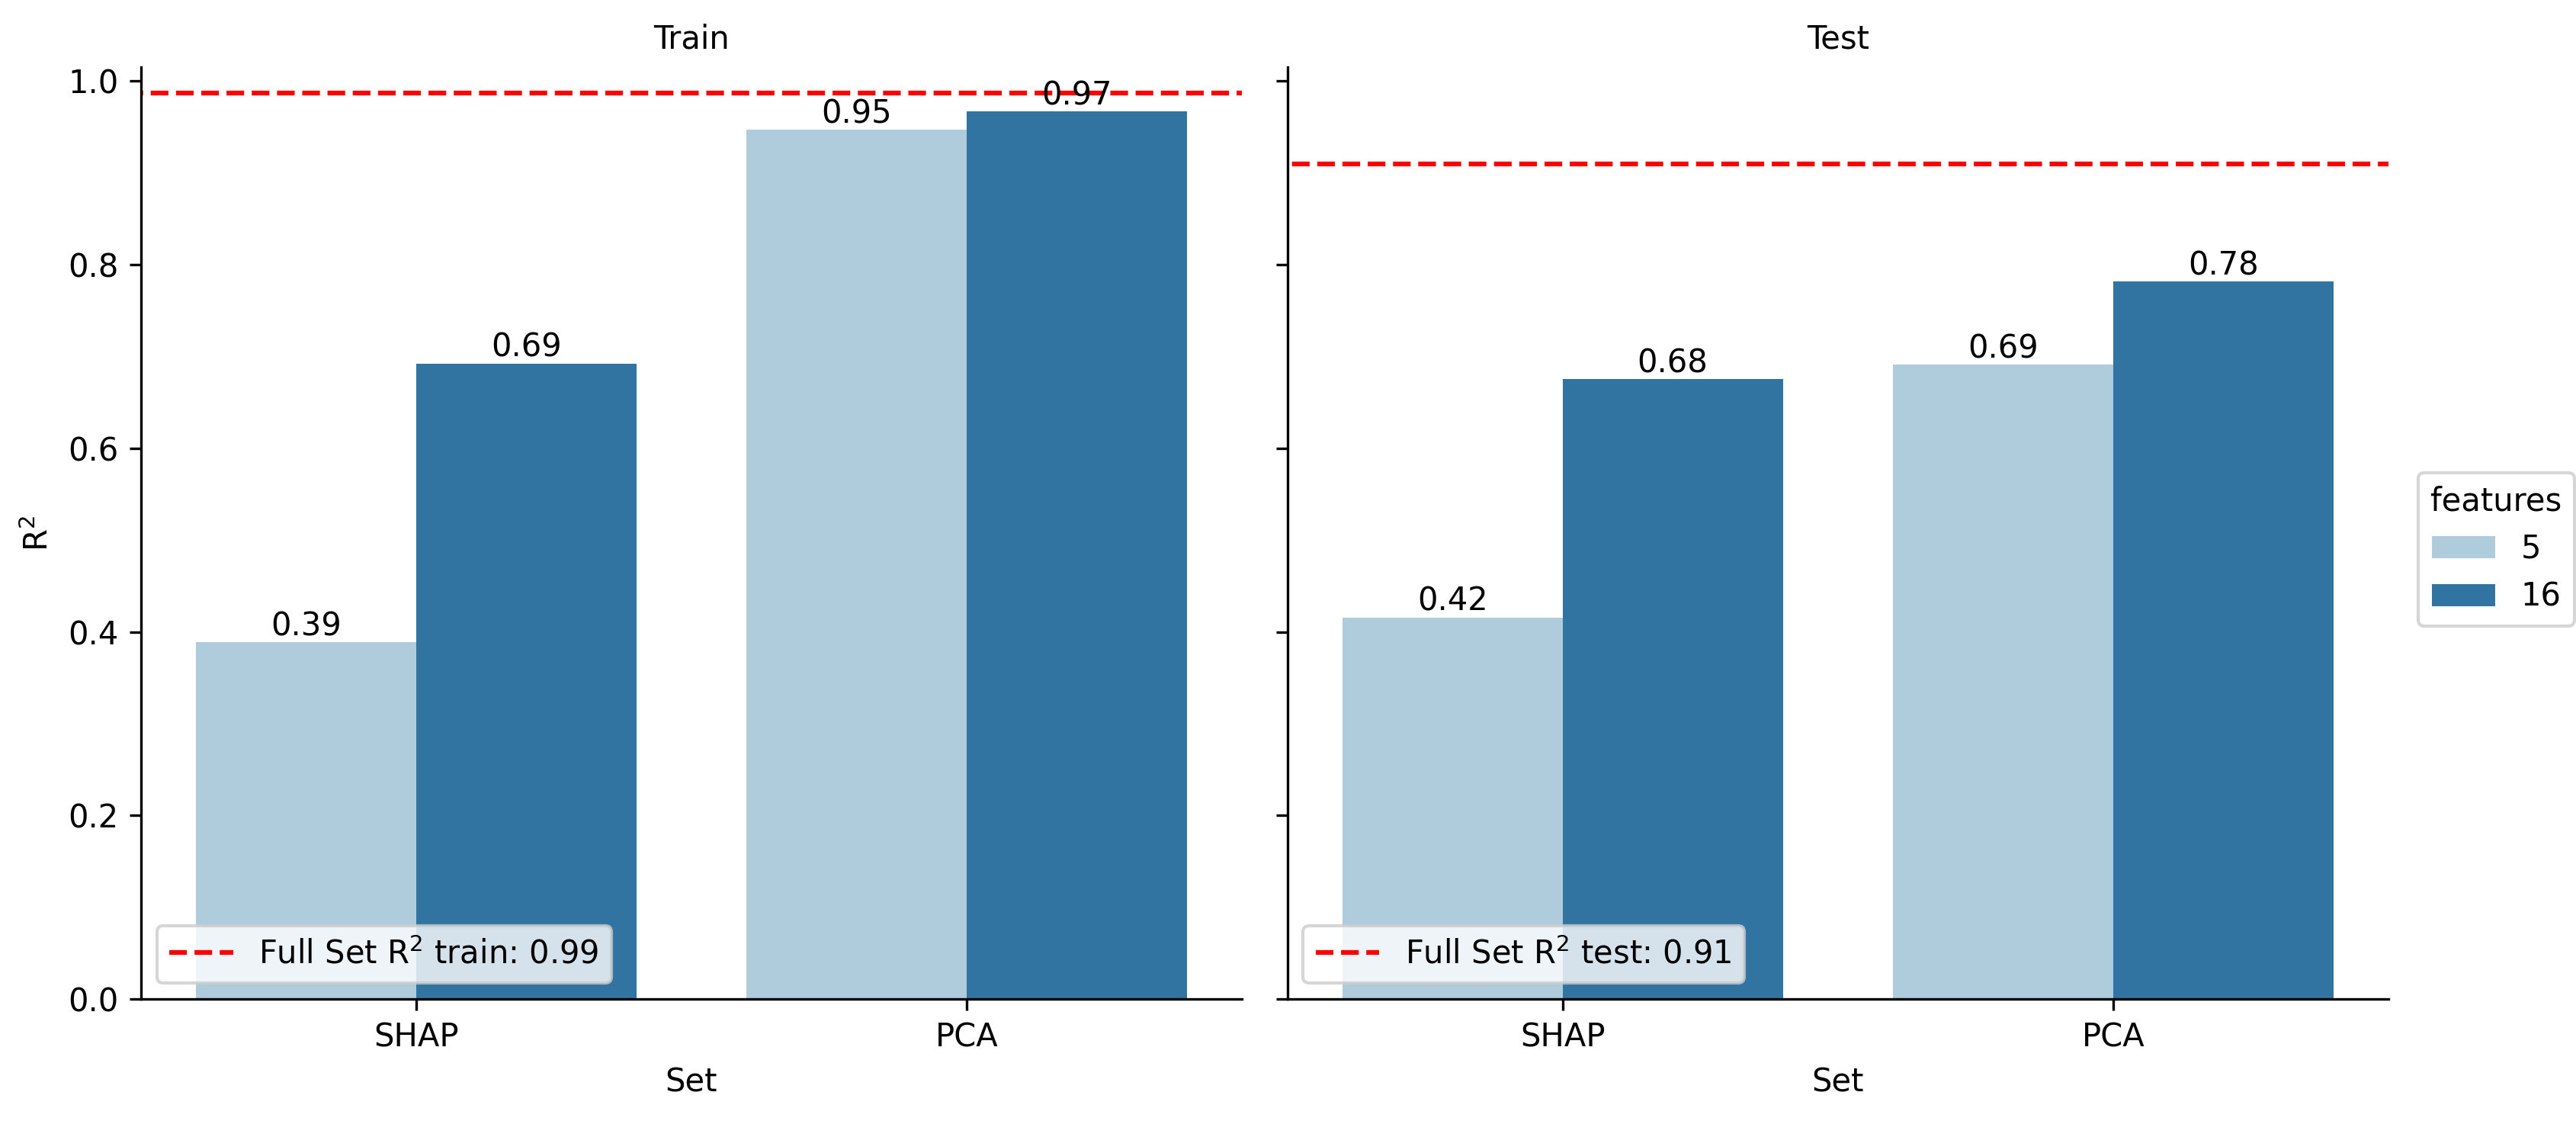
\includegraphics[width=\textwidth]{../images/BSE/classical_features_R2.png}
		\caption{}
		\label{fig:BSE_classical_features_R2}
	\end{subfigure}
	\caption{Feature reduction of the BSE dataset represented using }
	\label{fig:bse_classical_features}
\end{figure}

\begin{figure}[H]
	\centering
	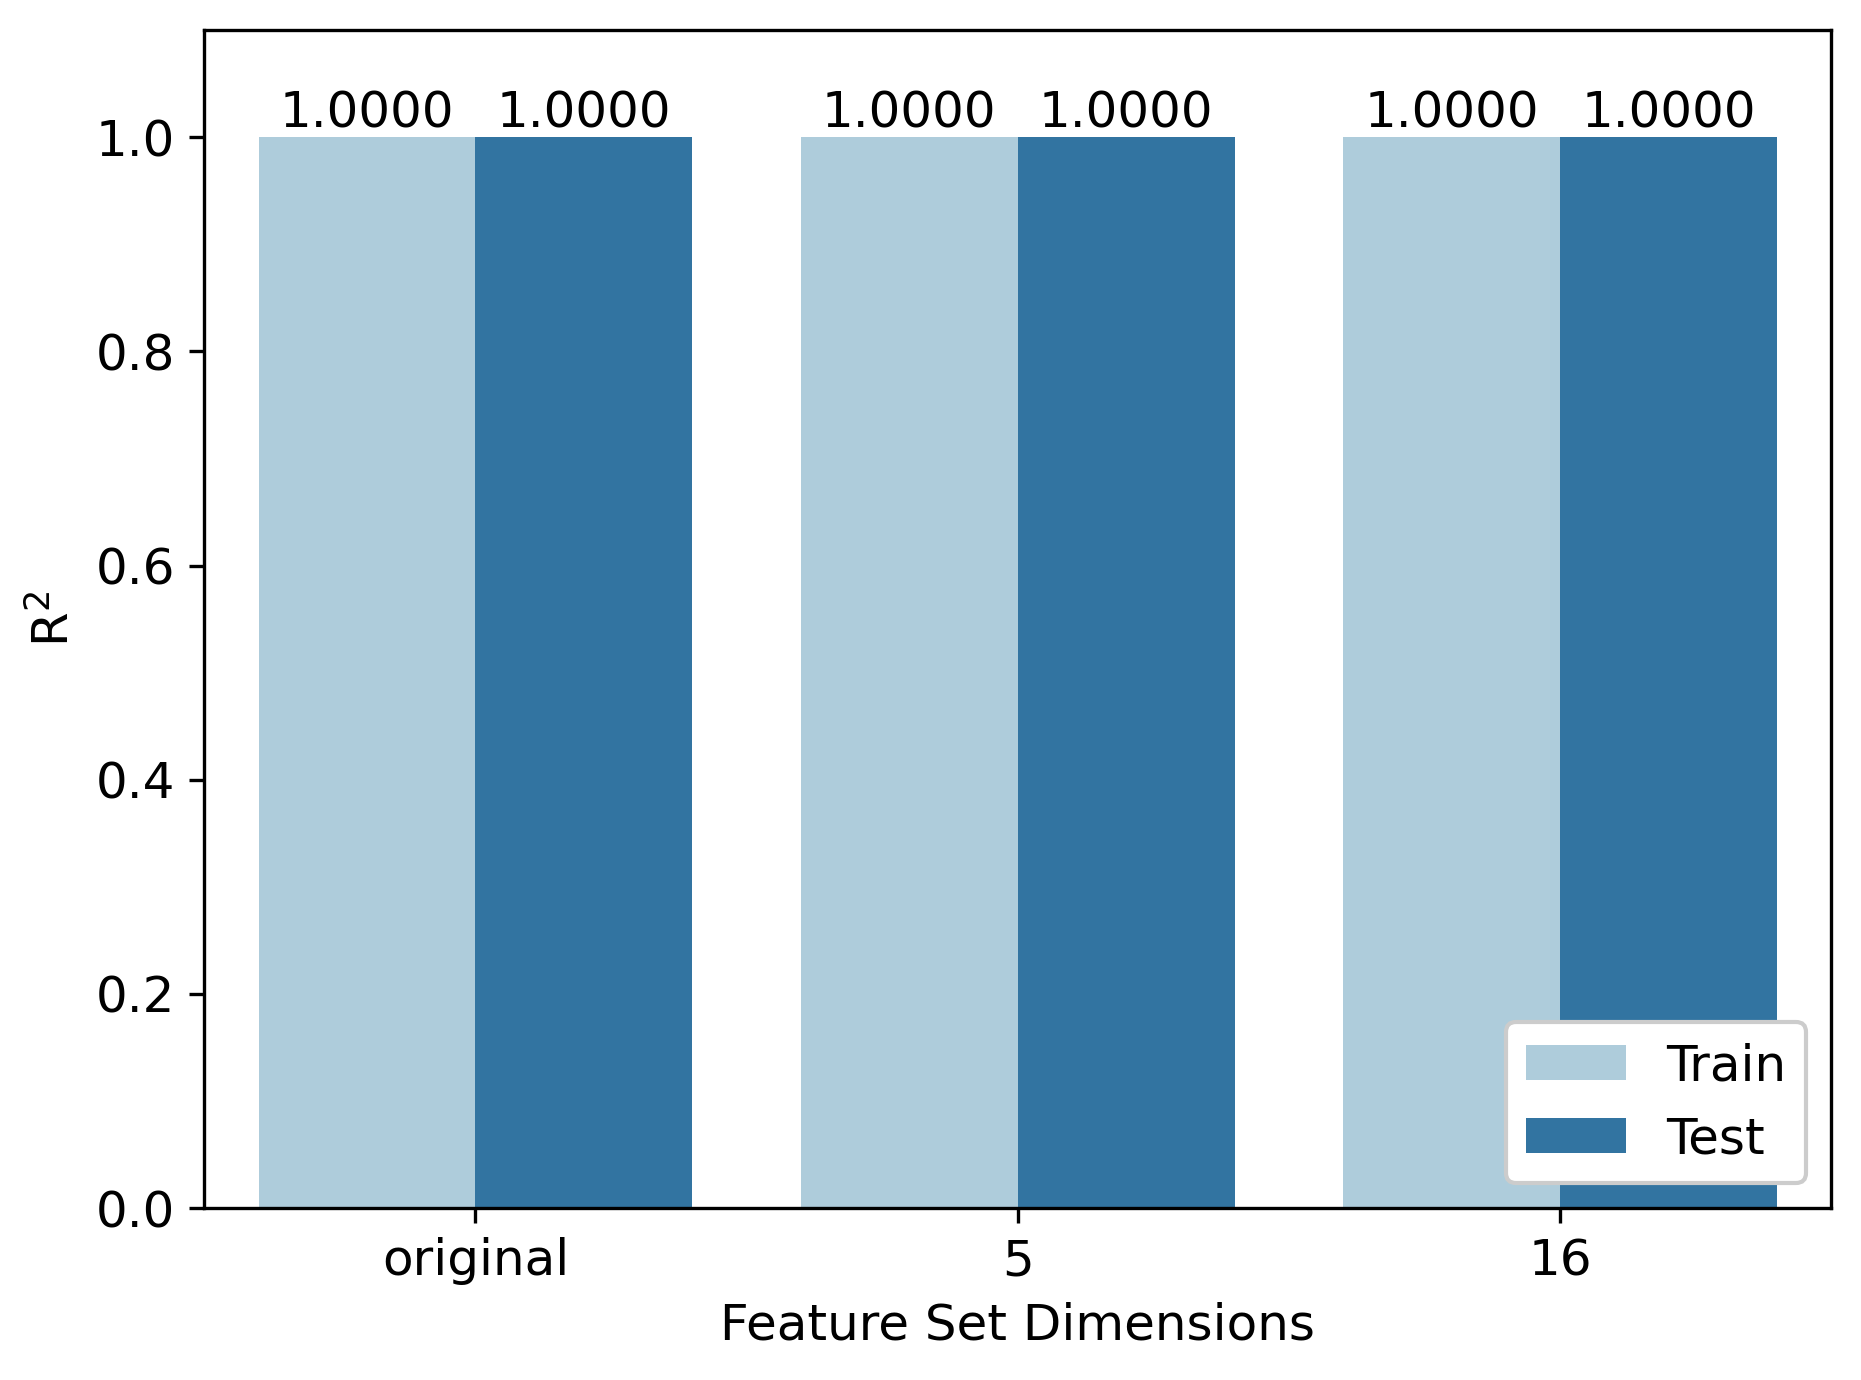
\includegraphics[width=0.49\textwidth]{../images/DDCC/DDCC_feature_set.png}
	\caption{}
	\label{fig:DDCC_feature_set}
\end{figure}

\section{DDCC Fake Quebec}\label{section:DDCC_fake}
Ran using the state vector model parameters for one iteration to test the optimization and resilience levels using Fake Quebec before running on the real device

\begin{figure}[H]
	\centering
	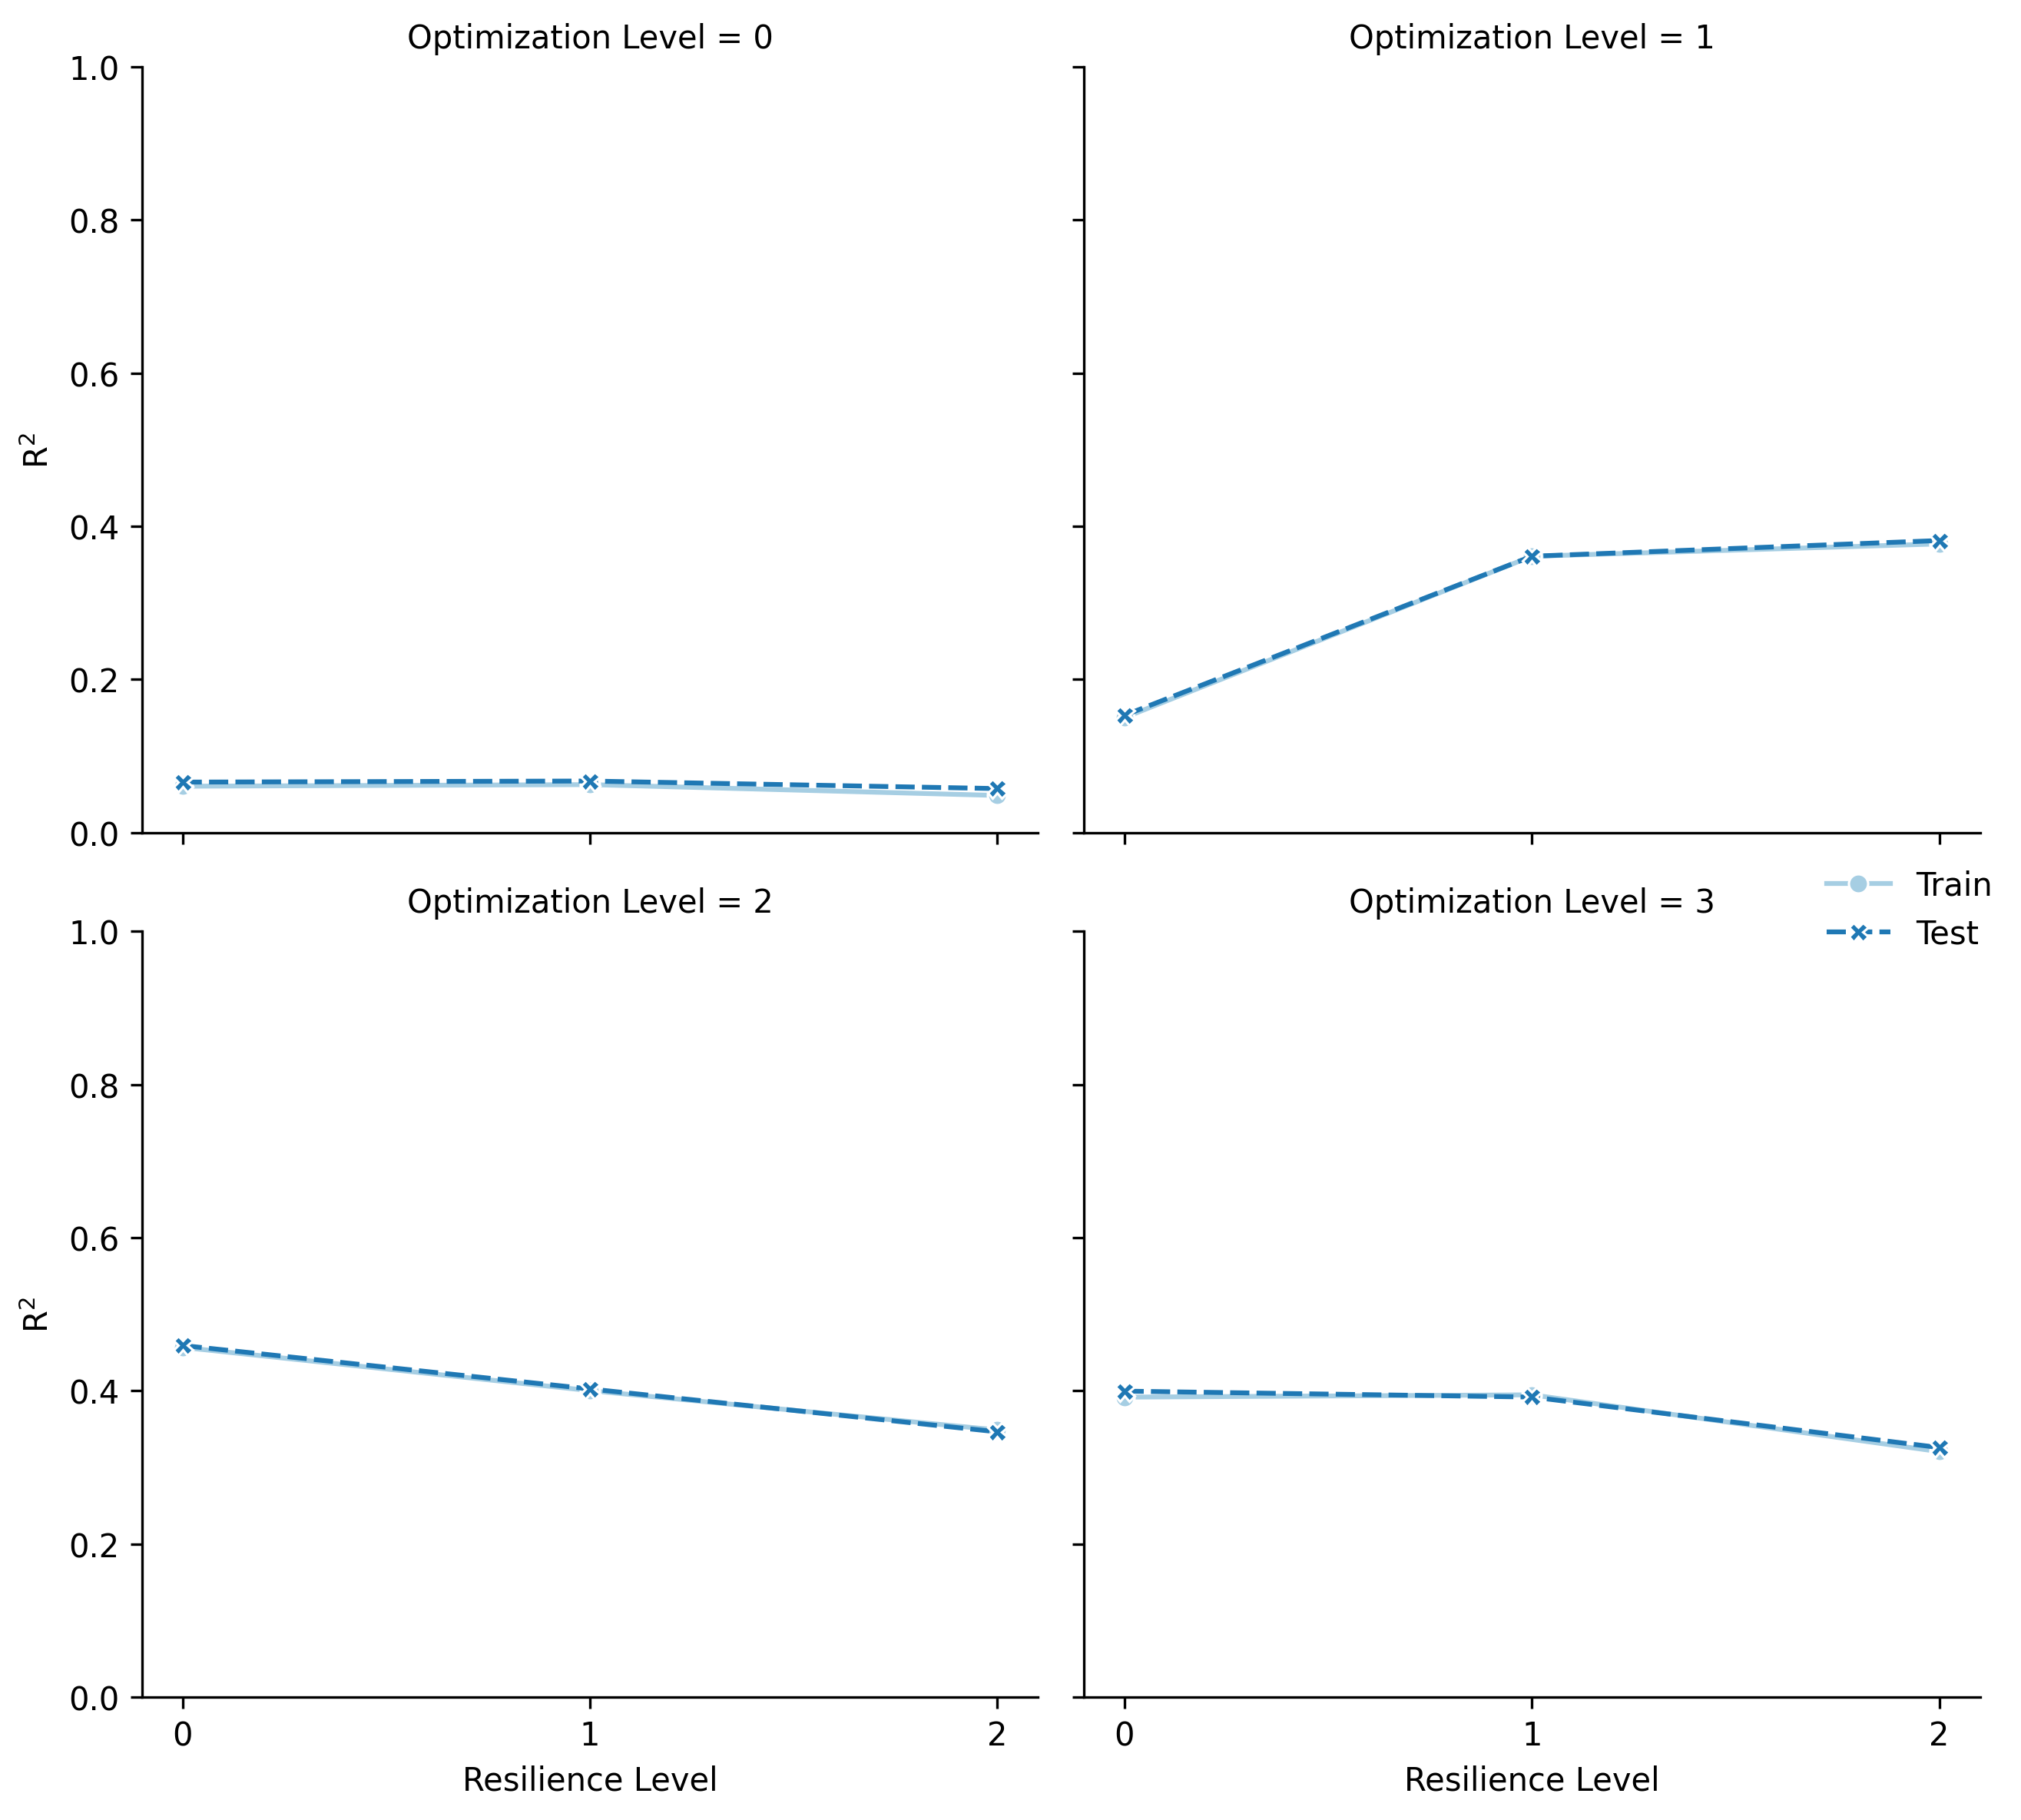
\includegraphics[width=1\linewidth]{../images/DDCC/opt_res_fakequebec}
	\caption{}
	\label{fig:optresfakequebec}
\end{figure}

\begin{figure}[H]
	\centering
	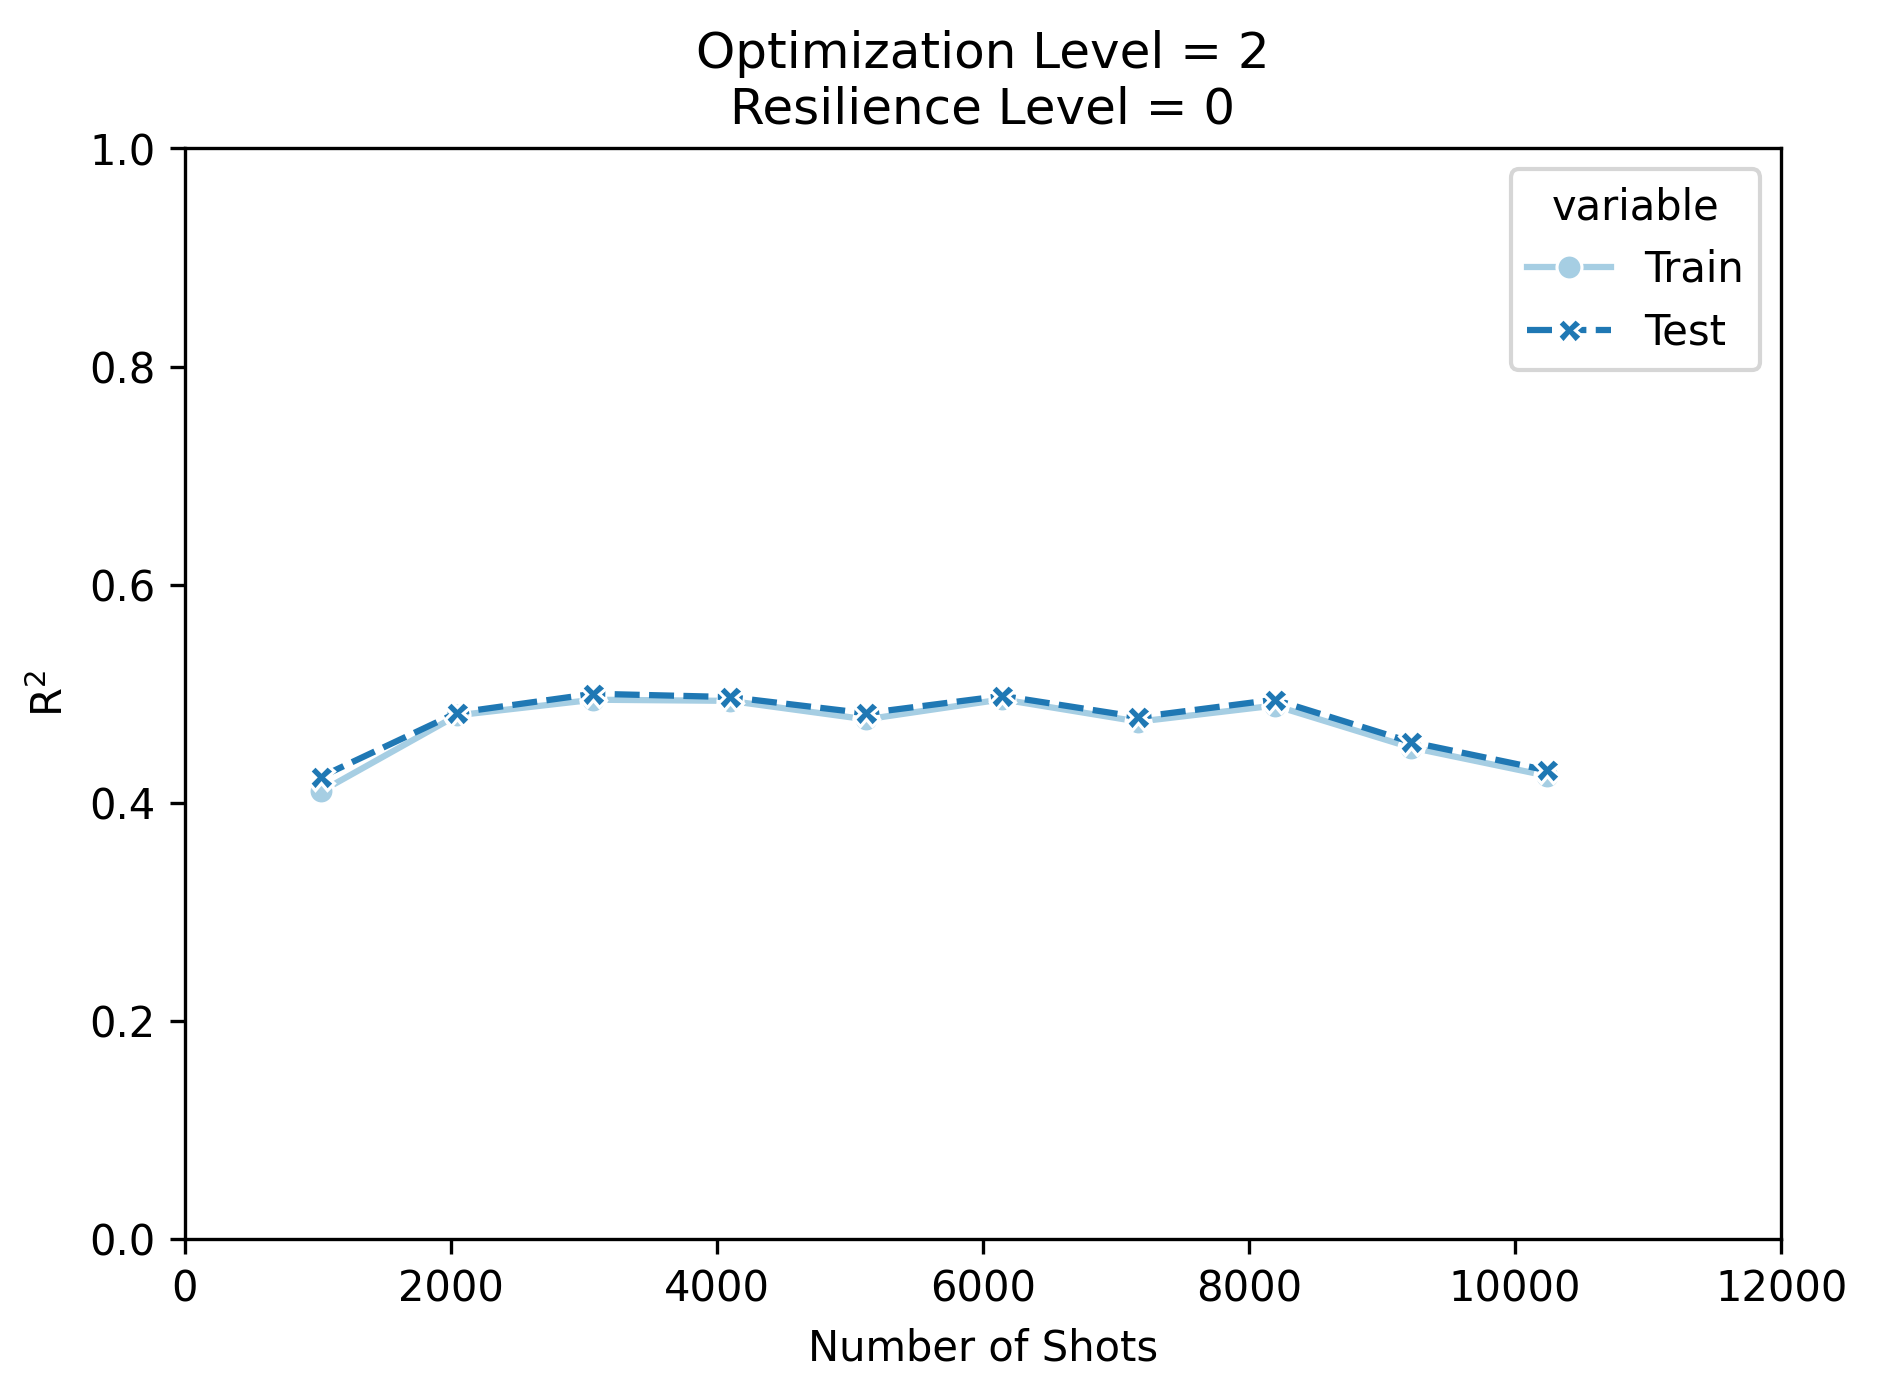
\includegraphics[width=1\linewidth]{../images/DDCC/shots_fakequebec}
	\caption{}
	\label{fig:shotsfakequebec}
\end{figure}



\section{title}\label{section:section3}












\end{document}